\documentclass[11pt, dvipsnames, handout]{beamer}
\newtoggle{full}
\settoggle{full}{true}

\newtoggle{covered}
\settoggle{covered}{false}

\newtoggle{presentable}
\settoggle{presentable}{false}

\newtoggle{dualscreen}
\settoggle{dualscreen}{false}

\usepackage{pgfplots}
%\pgfplotsset{compat = newest}

\usepackage{pgfpages}

\setbeamertemplate{note page}{\pagecolor{yellow!5}\vfill \insertnote \vfill}
\usepackage{collect}
\definecollection{notes}
\newcounter{notestaken}

\usepackage{xpatch}

\usepackage{ulem}

\usepackage[framemethod=tikz]{mdframed}

\usepackage{scalerel}
\usepackage{calc}

%\usepackage{enumitem}
\setlength\fboxsep{.2em}

\usepackage{graphicx} % Allows including images
\usepackage{booktabs} % Allows the use of \toprule, \midrule and \bottomrule in tables

\xpatchcmd{\itemize}
  {\def\makelabel}
  {\setlength{\itemsep}{0.65 em}\def\makelabel}
  {}
  {}


\xpatchcmd{\beamer@enum@}
  {\def\makelabel}
  {\setlength{\itemsep}{0.65 em}\def\makelabel}
  {}
  {}


%\makeatletter
%\renewcommand{\itemize}[1][]{%
%  \beamer@ifempty{#1}{}{\def\beamer@defaultospec{#1}}%
%  \ifnum \@itemdepth >2\relax\@toodeep\else
%    \advance\@itemdepth\@ne
%    \beamer@computepref\@itemdepth% sets \beameritemnestingprefix
%    \usebeamerfont{itemize/enumerate \beameritemnestingprefix body}%
%    \usebeamercolor[fg]{itemize/enumerate \beameritemnestingprefix body}%
%    \usebeamertemplate{itemize/enumerate \beameritemnestingprefix body begin}%
%    \list
%      {\usebeamertemplate{itemize \beameritemnestingprefix item}}
%      {%
%        \setlength\topsep{1em}%NEW
%        \setlength\partopsep{1em}%NEW
%        \setlength\itemsep{1em}%NEW
%        \def\makelabel##1{%
%          {%
%            \hss\llap{{%
%                \usebeamerfont*{itemize \beameritemnestingprefix item}%
%                \usebeamercolor[fg]{itemize \beameritemnestingprefix item}##1}}%
%          }%
%        }%
%      }
%  \fi%
%  \beamer@cramped%
%  \raggedright%
%  \beamer@firstlineitemizeunskip%
%}
%
%
%
%
%
%\makeatother

%\setlist[beamer@enum@]{topsep=1 em}
%\let\origcheckmark\checkmark %screw you dingbat
%\let\checkmark\undefined %screw you dingbat
%\usepackage{dingbat} 
%\let\checkmark\origcheckmark %screw you dingbat






%\usepackage{fontawesome}

\usepackage{mathtools}
\usepackage{etoolbox, calculator}

\usepackage{xcolor}
\usepackage{tikz}
\usetikzlibrary{arrows.meta}
\usetikzlibrary{calc}
\usepackage[nomessages]{fp}
\usepackage{transparent}
\usepackage{accsupp}
%\usepackage{color, xcolor}

%colorblind-friendly palette
%\definecolor{dblue}{RGB}{51,34,136}
\definecolor{lblue}{RGB}{136,204,238}
%\definecolor{green}{RGB}{17,119,51}
\definecolor{tan}{RGB}{221,204,119}
%\definecolor{mauve}{RGB}{204,102,119}

\usepackage{tcolorbox}



\usepackage{xifthen}
\usepackage{nicefrac}
\usepackage{amsmath}
\usepackage{amsthm}
\usepackage{amssymb}
\theoremstyle{definition}
\newtheorem*{define}{Definition}
\newtheorem*{recall}{Recall}


\DeclareMathOperator{\tr}{tr}

\usepackage{multicol}
%\setlength{\columnsep}{1cm}

\usepackage{tablists, amsmath,vwcol, cancel, polynom}
\usetikzlibrary{shapes, patterns, decorations.shapes}
%\usepackage{tikzpeople}
\tikzstyle{vertex}=[shape=circle, minimum size=2mm, inner sep=0, fill]
\tikzstyle{opendot}=[shape=circle, minimum size=2mm, inner sep=0, fill=white, draw]

% common math quick commands
\newcommand{\nicedd}[2]{\nicefrac{\text{d}#1}{\text{d}#2}}
\newcommand{\dd}[2]{\dfrac{\text{d}#1}{\text{d}#2}}
\newcommand{\pd}[2]{\dfrac{\partial #1}{\partial#2}}
\renewcommand{\d}[1]{\text{d}#1}
\newcommand{\ddn}[3]{\dfrac{\text{d}^{#3}#1}{\text{d}#2^{#3}}}
\newcommand{\pdn}[3]{\dfrac{\partial^{#3}#1}{\partial#2^{#3}}}
\newcommand{\p}[0]{^{\prime}}
\newcommand{\pp}[0]{^{\prime\prime}}
\newcommand{\op}[2][\text{L}]{#1 \left[ #2 \right]}

\newcommand{\lap}[1]{\mathcal{L}\left\{#1\right\}}
\newcommand{\lapinv}[1]{\mathcal{L}^{-1}\left\{#1\right\}}
\newcommand{\lapint}[1]{\int_0^\infty e^{-st}#1dt}
\newcommand{\evalat}[2]{\Big|_{#1}^{#2}}

\newcommand{\paren}[1]{ \left( #1 \right)}

\newcommand{\haxis}[4][\normcolor]{\draw[#1, <->] (-#2,0)--(#3,0) node[right]{$#4$}; }


\newcommand{\axis}[4]{\draw[\normcolor, <->] (-#1,0)--(#2,0) 
node[right]{$x$};
\draw[help lines, <->] (0,-#3)--(0,#4) node[above]{$y$};}

\newcommand{\laxis}[6]{\draw[<->] (-#1,0)--(#2,0) 
node[right]{$#5$};
\draw[ <->] (0,-#3)--(0,#4) node[above]{$#6$};}
\newcommand{\xcoord}[2]{
	\draw (#1,.2)--(#1,-.2) node[below]{$#2$};}
\newcommand{\textnode}[3]{
	\draw (#1,#2) node[below]{$#3$};}
	
\newcommand{\nxcoord}[2]{
	\draw (#1,-.2)--(#1,.2) node[above]{$#2$};}
\newcommand{\ycoord}[2]{
	\draw (.2,#1)--(-.2,#1) node[left]{$#2$};}
\newcommand{\nycoord}[2]{
	\draw (-.2,#1)--(.2,#1) node[right]{$#2$};}
\newcommand{\dlim}{\displaystyle\lim}
\newcommand{\dlimx}[1]{\displaystyle\lim_{x \rightarrow #1}}
\newcommand{\stickfig}[2]{
	\draw (#1,#2) arc(-90:270:2mm);
	\draw (#1,#2)--(#1,#2-.5) (#1-.25,#2-.75)--(#1,#2-.5)--(#1+.25,#2-.75) (#1-.2,#2-.2)--(#1+.2,#2-.2);}	

%\newcounter{example}
%\setcounter{example}{1}
%\newcounter{preFrameExample}
%\AtBeginEnvironment{frame}{\setcounter{preFrameExample}{\value{example}}}
%\newcommand{\ex}[1]{
%	 \setcounter{example}{\value{preFrameExample}}
%	 \textcolor{green}{\small\fbox{Example \arabic{example}: #1}}\\[8pt]
%	\stepcounter{example}}
%\newcommand{\exans}[1]{
%	\SUBTRACT{\value{preFrameExample}}{1}{\n}
%	 \textcolor{green}{\small\fbox{Solution \n: #1}}\\[8pt]}
\mode<presentation> {

% The Beamer class comes with a number of default slide themes
% which change the colors and layouts of slides. Below this is a list
% of all the themes, uncomment each in turn to see what they look like.


\usetheme{CambridgeUS}
\usecolortheme[named=black]{structure}


\newcommand{\studentcolor}[0]{ForestGreen}
\newcommand{\normcolor}[0]{NavyBlue}
\newcommand{\alertcolor}{Red}

\setbeamercolor{normal text}{fg=\normcolor}
\setbeamercolor{frametitle}{fg=\normcolor}
\setbeamercolor{section in head/foot}{fg=Black, bg=Gray!20}
\setbeamercolor{subsection in head/foot}{fg=Green!70!Black, bg=Gray!10}
\setbeamercolor{alerted text}{fg=\alertcolor}
\setbeamerfont{alerted text}{series=\bf}
\setbeamertemplate{enumerate items}[default]
\setbeamercolor{enumerate item}{fg=\normcolor}

\setbeamertemplate{footline} % To remove the footer line in all slides uncomment this line
%\setbeamertemplate{footline}[page number] % To replace the footer line in all slides with a simple slide count uncomment this line

\setbeamertemplate{navigation symbols}{} % To remove the navigation symbols from the bottom of all slides uncomment this line
}

\newcommand{\alertbox}[1]{\tcbox[on line, colframe=\alertcolor, colback=White, left=2pt,right=2pt,top=2pt,bottom=2pt]{\usebeamercolor*{normal text}#1}}


\newcommand{\startstu}{\setbeamercolor{normal text}{fg=\studentcolor}\usebeamercolor*{normal text}\setbeamercolor{enumerate item}{fg=\studentcolor}\usebeamercolor*{enumerate item}}
\newcommand{\stopstu}{\setbeamercolor{normal text}{fg=\normcolor}\usebeamercolor*{normal text}\setbeamercolor{enumerate item}{fg=\normcolor}\usebeamercolor*{enumerate item}}

\newcommand{\takenote}[1]{ \begin{collect}{notes}{}{}{}{}  #1  \end{collect}  \addtocounter{notestaken}{1}} %\ifthenelse{\value{notestaken}>0}{\hrulefill\\}{}

\makeatletter
\newcommand{\cover}{\alt{\beamer@makecovered}{\beamer@fakeinvisible}}
\newcommand{\ucover}[1]{\iftoggle{full}{}{\beamer@endcovered}\stopstu#1\startstu\iftoggle{full}{}{\beamer@startcovered}}
\makeatother

\newcommand{\skippause}{ \addtocounter{beamerpauses}{-1}}
\newcommand{\blockpres}{ \skippause \pause }

\newcommand{\studentify}[1]{\startstu #1  \stopstu }
\newcommand{\student}[1]{\iftoggle{full}{ \pause  \studentify{#1} }{\iftoggle{covered}{\studentify{#1}}{\cover{  #1 }}}}
\newcommand{\cstudent}[1]{\student{\begin{center} #1 \end{center}}}
\newcommand{\fullonly}[1]{\iftoggle{full}{ #1}{}}
\newcommand{\presentonly}[1]{\iftoggle{presentable}{ #1}{}}

\usepackage{xparse}
\usepackage{xifthen}

% shortcuts for commonly-used presentation elements
%\NewDocumentCommand{\slide}{o m}
% {\IfValueTF{#1}{\begin{frame}[t]{#1}}{\begin{frame}[t]} #2 \end{frame}}

\newtoggle{iscovered}

\newcommand{\slide}[2][]{%
%\setcounter{notestaken}{0}
\takenote{#2} 
%\ifthenelse{\equal{#1}{}}{\begin{frame}[t]}{\begin{frame}[t]{#1}} #2 \ifthenelse{\value{notestaken}>0}{ \note{\includecollection{notes}}}{} \end{frame}%
\ifthenelse{\equal{#1}{}}{\begin{frame}[t]}{\begin{frame}[t]{#1}} #2 \iftoggle{covered}{\settoggle{iscovered}{true}}{\settoggle{iscovered}{false}}  \note{ \iftoggle{iscovered}{}{\settoggle{covered}{true}} #2 \iftoggle{iscovered}{}{\settoggle{covered}{false}} } \end{frame}%
%\setcounter{notestaken}{0}
}
\newcommand{\defn}[2][]{%
 \setcounter{listcounter}{0}%
\ifthenelse{\equal{#1}{}}{\begin{block}{Definition}}{\begin{block}{#1 :}}%
 #2 \vspace{0.25em} \ifthenelse{\value{listcounter}>0}{\skippause}{} \pause \end{block}%
}



\newcommand{\arr}[2]{\begin{array}{#1}#2\end{array}}
\newcommand{\mat}[2]{\left[\arr{#1}{#2}\right]}
\newcommand{\carray}[1]{\arr{c}{#1}}
\newcommand{\larray}[1]{\arr{l}{#1}}
\newcommand{\rarray}[1]{\arr{r}{#1}}
\newcommand{\colvec}[1]{\mat{c}{#1}}

\newcommand{\itmz}[1]{\addtocounter{listcounter}{1} \begin{itemize}#1 \end{itemize} }
\newcommand{\subitem}[1]{\addtocounter{listcounter}{1} \begin{itemize} \item #1 \end{itemize}}
%
\newcommand{\enum}[1]{\addtocounter{listcounter}{1} \begin{enumerate} #1  \end{enumerate}  }


\newcommand{\algnlbl}[1]{\begin{align}#1  \end{align}} 
\newcommand{\algn}[1]{\begin{align*}#1  \end{align*}} 
\newcommand{\lgn}[1]{ \action<+->{#1} }
\newcommand{\slgn}[1]{\iftoggle{full}{\action<+->{ \startstu #1 \stopstu}}{ \cover{ #1 } } \takenote{$#1$}}

\newcommand{\chckmrk}{\alert{\checkmark}}

\usepackage{pifont}
\newcommand{\xmark}{\alert{\text{\large \ding{55}}}}

\newcommand{\return}[0]{\raisebox{.5ex}{\rotatebox[origin=c]{180}{$\Lsh$}}}
\usepackage{pbox}
%\newcommand{\ex}[1]{\rotatebox[origin=c]{10}{\uline{ex}}:$\;$\pbox[t][][b]{0.9\linewidth}{#1}}
\newcommand{\ex}[1]{\uline{ex}:$\;$\pbox[t][][t]{0.9\linewidth}{#1}}
\newcommand{\eg}[1]{e.g.,$\;$\pbox[t][][t]{0.9\linewidth}{#1}}
\newcommand{\tikzplot}[8][]{%
\begin{tikzpicture}

\begin{scope}[]%
\clip(-#2,-#4) rectangle (#3,#5);%
#8%
\end{scope}%
\laxis{#2}{#3}{#4}{#5}{#6}{#7}%
#1
\end{tikzpicture}%
}


\newcommand{\cancelslide}[1]{%
\begingroup%
\setbeamertemplate{background canvas}{%
\begin{tikzpicture}[remember picture,overlay]%
\draw[line width=2pt,red!60!black] %
  (current page.north west) -- (current page.south east);%
\draw[line width=2pt,red!60!black] %
  (current page.south west) -- (current page.north east);%
\end{tikzpicture}}%
#1%
\endgroup%
}
\renewcommand{\CancelColor}{\color{red}}
\newcommand{\twocols}[3][0.5]{\begin{columns}\begin{column}{#1\textwidth}#2\end{column}\hspace{1em}\vrule{}\hspace{1em}\begin{column}{#1\textwidth}#3\end{column}\end{columns}}

\newcommand{\twomini}[5][1]{\calculatespace \begin{minipage}[t]{\columnwidth}\begin{minipage}[][#1\contentheight][t]{#2\columnwidth}#4\end{minipage}\hfill\begin{minipage}[][#1\contentheight][t]{#3\columnwidth}#5\end{minipage}\end{minipage}}

\newcommand{\threemini}[7][1]{\calculatespace \begin{minipage}[t]{\columnwidth}\begin{minipage}[][#1\contentheight][t]{#2\columnwidth}#5\end{minipage}\hfill\begin{minipage}[][#1\contentheight][t]{#4\columnwidth}#6\end{minipage}\hfill\begin{minipage}[][#1\contentheight][t]{#3\columnwidth}#7\end{minipage}\end{minipage}}


\newcounter{listcounter}
\setcounter{listcounter}{0}



\newif\ifsidebartheme
\sidebarthemetrue

\newdimen\contentheight
\newdimen\contentwidth
\newdimen\contentleft
\newdimen\contentbottom
\makeatletter
\newcommand*{\calculatespace}{%
\contentheight=\paperheight%
\ifx\beamer@frametitle\@empty%
    \setbox\@tempboxa=\box\voidb@x%
  \else%
    \setbox\@tempboxa=\vbox{%
      \vbox{}%
      {\parskip0pt\usebeamertemplate***{frametitle}}%
    }%
    \ifsidebartheme%
      \advance\contentheight by-1em%
    \fi%
  \fi%
\advance\contentheight by-\ht\@tempboxa%
\advance\contentheight by-\dp\@tempboxa%
\advance\contentheight by-\beamer@frametopskip%
\ifbeamer@plainframe%
\contentbottom=0pt%
\else%
\advance\contentheight by-\headheight%
\advance\contentheight by\headdp%
\advance\contentheight by-\footheight%
\advance\contentheight by4pt%
\contentbottom=\footheight%
\advance\contentbottom by-4pt%
\fi%
\contentwidth=\paperwidth%
\ifbeamer@plainframe%
\contentleft=0pt%
\else%
\advance\contentwidth by-\beamer@rightsidebar%
\advance\contentwidth by-\beamer@leftsidebar\relax%
\contentleft=\beamer@leftsidebar%
\fi%
}
\makeatother



\iftoggle{dualscreen}{\setbeameroption{show notes on second screen=right}}{}

\settoggle{covered}{true}
\begin{document}
\section{Introduction}
\subsection{Overview}
\slide[Differential Equations]{
\vfill
\enum{

\item What are they and why do we solve them?
\item Terminology
\item Graphical intuition and the direction field
}\vfill
}
\subsection{Preliminaries}
\slide[What is a Differential Equation?]{\vspace{-.5em}
A differential equation (DE) is an equation involving an unknown function $y$ and atleast one derivative of $y$ w.r.t. an independent variable.
\vfill
\twomini[.8]{.02}{.98}{\hspace{.15cm}}{\itmz{
\item [Given:]  A DE with an unknown function $y(t)$. \hfill  \student{e.x., $\carray{\dd{y}{t} = - 3 y(t) \\ \text{\uline{or}} \\ \\y\p = -3y}$}
\item[Task:]  Find the function(s) $y(t)$.\hfill  \student{Solution: $y(t)=C_1e^{-3t}$}
\vfill
\item[Tools:]
\itmz{\item Calculus (i.e., integration/differentiation) \item Guess and check (does some function $f(t)$ make LHS=RHS?) \item Specialized procedures (informed by experience geussing) \item Geometry/Linear Algebra (useful for systems of DEs)}
}
}
}

\slide[Example: Skydiving \hfill\begin{minipage}{0.25\textwidth}{ 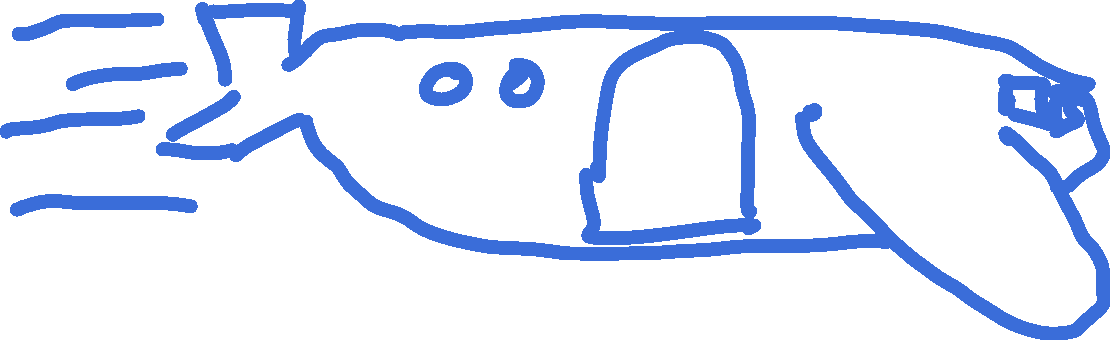
\includegraphics[height=1cm]{images/airplane.pdf}}\end{minipage} ]{
\begin{center}
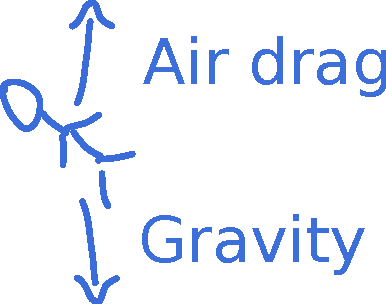
\includegraphics[height=2cm]{images/skydiver_solo.pdf}
\end{center}
Newton's Second Law:\[F=ma\]
\student{\algn{
ma &= \underbrace{-mg}_{\text{gravitational force}} \hspace{2em} \underbrace{-\mu v}_{\text{drag force}}\\
a&=v'\\
\Aboxed{mv' &= -mg - \mu v} \qquad \text{DE for } v(t)
}
}
}

\slide[Example: Epidemiology]{
Kermack \& McKendrick's SIR model\subitem{
\uline{S}usceptible $\rightarrow$ \uline{I}nfected $\rightarrow$ \uline{R}ecovered}
\vfill
System of 3 ordinary differential equations:
\twomini[.4]{.65}{.33}{
\algn{
\dd{S}{t} & = \mu (I+R)  - \beta SI \\
\dd{I}{t} &= \beta SI - \gamma  I - \mu I\\
 \dd{R}{t} &= \gamma I - \mu R
}
}{
\algn{
t & = \text{time}\\
\beta & =\text{infection rate}\\
\gamma &=\text{recovery rate}\\
\mu &= \text{birth/death rate}
}
}
\vfill
Reproduction number: $R_0=\frac{\beta}{\mu+\gamma}$
\enum{\item $R_0>1$: endemic equilibrium \item $R_0<1$: disease dies out \hfill - \hfill basic idea behind "flatten the curve"}
}

\subsection{Terminology}


\slide[Terminology: ODEs vs PDEs]{
\itmz{
\item Ordinary differential equation (ODE) \student{\hfill (covered in this course)}
\student{\subitem{A DE with derivatives w.r.t. only one independent variable. \vfill\item $\dd{y}{t} = y(t) + 3 \qquad \text{or} \qquad \dd{y}{t} = \sin(y) + \cos(t) $ }}\vfill
\item Partial differential equation (PDE) \student{\hfill (not covered in this course)}
\student{\subitem{A DE with derivatives w.r.t multiple independent variable. \vfill
\item Heat/Diffusion eq: $\pd{u}{t} = D\pdn{u}{x}{2}$\vfill
\item Wave eq: $\pdn{u}{t}{2} = c \pdn{u}{x}{2}$\vfill
\item Partial derivatives are necessary for solutions to agree when changing coordinate systems (e.g., switch from cartesian to polar coordinates)
}}
}
}


\slide[Terminology: Order of a DE]{
The highest derivative that appears in the DE.
\itmz{
\item $y\p=y+3$ \hspace{2em} \student{first order}
\item  $y\p=y^2+9$  \hspace{2em} \student{first order}
\item  $\left(\dd{y}{t}\right)^2=\tan(t)$  \hspace{2em} \student{first order}
\item  $y\pp=-y$  \hspace{2em} \student{second order}
\item  $\ddn{y}{x}{4}=ky$  \hspace{2em} \student{fourth order}
}
}

\slide[Terminology: Operator Form  \hfill $\Rightarrow$ \hfill $\op{y(t)} = f(t)$]{\vspace{-0.5em}
Everything that depends on the unknown function goes on one side of the equal sign and everything else on the other.\vfill
\subitem{ $\dd{y}{t} = y(t) + 3 \quad \to \quad \student{\dd{y}{t} - y(t) = 3}$ \vfill \student{\subitem{$\op{y}=f\p-y, \quad f(t) = 3$}}\vfill
\item  $\dd{y}{t} =\sin(y) + \cos(t) \quad \to \quad \student{\dd{y}{t} - \sin(y) = \cos(t)}$ \vfill \student{\subitem{$\op{y}=f\p-\sin(y), \quad f(t) = \cos(t)$}\vfill}
}
\vfill

The operator $\op{\cdot}$, encodes the "intrinsic" dynamics that the ODE is modelling.  \student{\subitem{Force-displacement relationship of a spring. \item Velocity-drag relationship of a viscous fluid.}}

}

\slide[Terminology: Linearity of DEs \hfill - \hfill $\op{y(t)} = f(t)$ ]{
If the operator $\op{\cdot}$ is linear, then the DE is linear.
\vfill
\uline{Conditions for linearity:}\vfill
Given any two functions $f$ and $g$ and a constant $c$, a linear operator satisfies

\enum{
\item\student{ $\op{f+g}=\op{f}+\op{g}$}\vfill
\item\student{ $\op{cf}=c\op{f}$}\vfill
}
\uline{In practice:} does the operator have any nonlinear functions?\vfill
\twomini[0.2]{0.5}{0.5}{
\ex{$\op{y}=y''+y$}\\~\\
\centering
\student{Linear}
}{
\ex{$\op{y}=y'+\sin(y)$}\\~\\
\centering
\student{Nonlinear}
}

}

\slide[Terminology: Autonomous DEs \hfill - \hfill $\op{y(t)} = f(t)$]{
If both $\op{\cdot}$ and $f(t)$ do not explicitly depend on the independent variable, then the DE is autonomous. \vfill 

\itmz{
\item $y\p=y$  \student{  $\to \quad y\p-y=0$ \hfill Autonomous}
\item  $y\p=y^2+3$   \student{  $\to \quad \dd{y}{t}-y^2=3$ \hfill Autonomous}
\item  $\dd{y}{t}=y+\tan(t)$   \student{  $\to \quad \dd{y}{t}-y=\tan(t)$ \hfill Non-autonomous}
\item  $\dd{y}{t}=-3ty$  \student{  $\to \quad \dd{y}{t}+3ty=0$ \hfill Non-autonomous}

}
\vfill
$f(t)$ is often called the (external) forcing term. \vfill \student{ constant or zero-forcing $\Rightarrow$ Autonomous DE }

}

\slide[Classifying ODEs]{
\itmz{\item $x\pp + x^2 = t$ \subitem{Order: \student{2} \item Linear: \student{No} \item Autnomous: \student{No}}\vfill
\item $\ddn{x}{t}{4} = 0$ \subitem{Order: \student{4} \item Linear: \student{Yes} \item Autnomous: \student{Yes}}
}
}
\slide[Terminology: Solution to an ODE]{
A solution of an ODE is a function that satisifes the ODE.\vfill
\ex{Is $y=Ce^{-t}+t-1$ a solution to $y\p+y=t$?}
\student{
\algn{y\p&=-Ce^{-t}+1\\
y\p+y&=\cancel{-Ce^{-t}}+\cancel{1} + \cancel{  Ce^{-t}}+t-\cancel{1}\\
&=t\quad \checkmark
}}Here $C$ is an arbitrary constant that can have any value.\vfill
Any solution with an arbitrary constant is called a \student{\uline{general solution}}
\vfill
We can obtain a unique solution by imposing some constaint, a solution with no arbitrary constants is called a \student{\uline{particular solution}}
 
\vfill
}

\slide[Initial Value Problems]{\vspace{-0.75em}
ODEs of the form\[\op{y} =f(t), \text{ with } y(t_0)=y_0,\] where $t_0$ and $y_0$ are numerical values (usually real-valued).
\vfill
\ex{Find the particular solution to $y\p+y=t$ with $y(0)=0$?}\vfill
\student{
Start with the general solution
\algn{y(t)&=Ce^{-t}+t-1\intertext{evaluate at $t=t_0=0$, make that equal to $y_0=0$}
y(0) &= C-1 = 0 \quad \Rightarrow C=1\\
\Aboxed{y(t) &=e^{-t}+t-1}}}
}

\slide[Summary]{
\enum{\item What are DEs?
\subitem{Equations involving unknown function(s) and function derivatives. \item Specify rates of change of certain quantities. \item Useful for modelling many natural phenomena.}\vfill
\item Terminology \subitem{ODEs (\& PDEs). 
\item Order of DEs, Linear DEs, Autonomous DEs, Solutions to DEs}\vfill
\item Initial Value Problems  \subitem{ The most "standard" way to obtain a unique solution \item Specify solution value at some initial time}
}

}
\end{document}